\section{Data types}
\label{sec:dtype}
\begin{frame}<beamer>
    \frametitle{Outline}
    \tableofcontents[currentsection]
\end{frame}


\begin{frame}{Data Types Supported in C}
\begin{figure}
	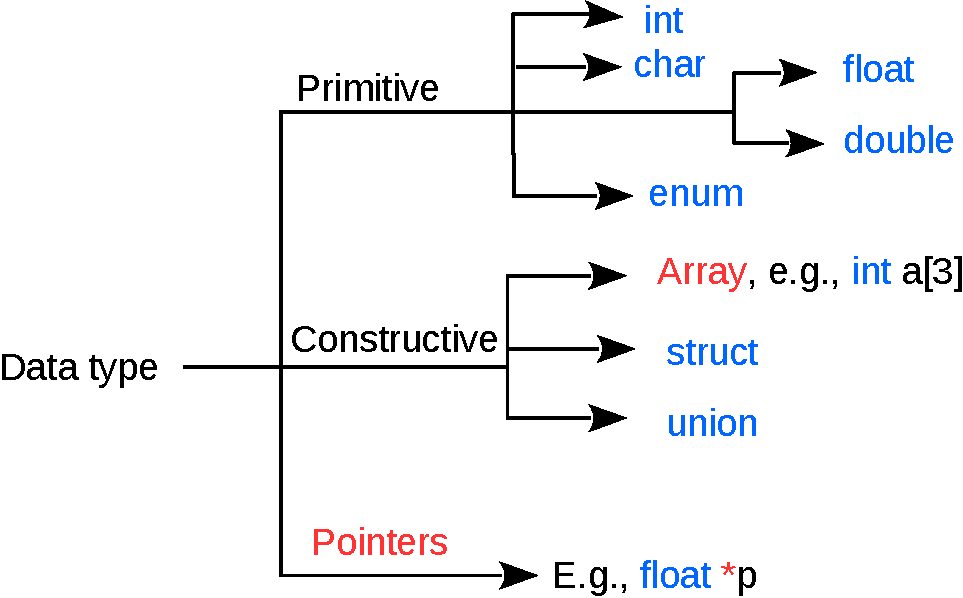
\includegraphics[width=0.75\linewidth]{figs/dtypes.pdf}
\end{figure}
\end{frame}

\begin{frame}[fragile]{Integer numbers}
	\begin{itemize}
		\item Keywords: \textcolor{blue}{int}, \textcolor{blue}{short}, \textcolor{blue}{long}
		\item Can be \textit{signed} (\textcolor{red}{default}) or \textit{unsigned}
		\item Actual size of \textit{int}, \textit{short}, \textit{long} depends on architecture
	\end{itemize}
	\begin{center}
	\begin{lstlisting}[language=c,frame=none, linewidth=0.85\linewidth]
 int a;	/*Range: -2,147,483,648 to 2,147,483,647*/
 short b;	/*Range: -32,768 to 32,767*/
 long c; /*Range: -2,147,483,648 to 2,147,483,647*/
 unsigned int a1;	/*Range: 0 to 4,294,967,297*/		
 unsigned short b1;	/*Range: 0 to 65,535*/
	\end{lstlisting}
	\end{center}	
	\begin{itemize}
		\item {\textcolor{blue}{int} and \textcolor{blue}{long} take 4 bytes (32 bits system)}
		\item {\textcolor{blue}{short} takes 2 bytes}
	\end{itemize}
\end{frame}

\begin{frame}[fragile]{Integer numbers}
	\vspace{-0.2in}
	\begin{itemize}
		\item Keywords: \textcolor{blue}{int}, \textcolor{blue}{short}, \textcolor{blue}{long}
		\item Can be \textit{signed} (\textcolor{red}{default}) or \textit{unsigned}
		\item Actual size of \textit{int}, \textit{short}, \textit{long} depends on architecture
	\end{itemize}
	%\vspace{-0.1in}
	\begin{figure}
		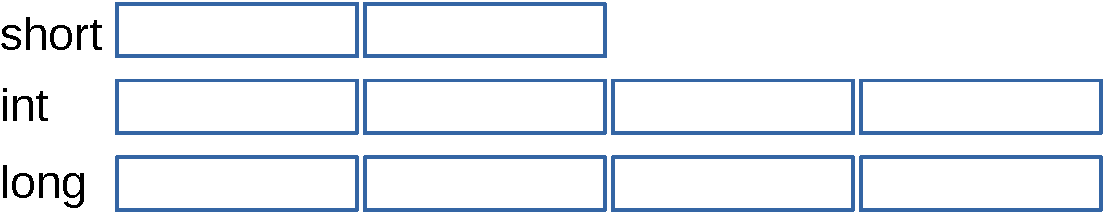
\includegraphics[width=0.65\linewidth]{figs/ints.pdf}
	\end{figure}
	\vspace{-0.1in}
	\begin{center}
	\begin{lstlisting}[language=c,frame=none, linewidth=0.9\linewidth]
 int a;	/*Range: -2,147,483,648 to 2,147,483,647*/
 short b;	/*Range: -32,768 to 32,767*/
 long c; /*Range: -2,147,483,648 to 2,147,483,647*/
 unsigned int a1;	/*Range: 0 to 4,294,967,297*/		
 unsigned short b1;	/*Range: 0 to 65,535*/
	\end{lstlisting}
	\end{center}	
\end{frame}


\begin{frame}[fragile]{Integer numbers}
	\begin{center}
		\begin{lstlisting}[numbers=none, frame=none, language=c]
	    int main()
	    {
	       short a = 0x8000;
	       short b = 0x7FFF;
	       short c = 0xFFFE;
	       char  d = 0x80;
	       printf("a = %d, b = %d, c = %d\n", a, b, c);
	       printf("d = %d\n", d);
	       return 0;
	    }
	\end{lstlisting}
	\end{center}	
\end{frame}

\begin{frame}[fragile]
	\frametitle{The Problem of Overflow (1)}
\begin{itemize}
	\item {Given following code, anything wrong??}
\end{itemize}
		\begin{lstlisting}[numbers=none, frame=none, language=c]
	    int main()
	    {
	       unsigned short b = 65537;
	       return 0;
	    }
	\end{lstlisting}
\end{frame}

\begin{frame}[fragile]
	\frametitle{The Problem of Overflow (2)}
\begin{itemize}
	\item {Given following code, anything wrong??}
\end{itemize}
		\begin{lstlisting}[numbers=none, language=c,frame=none]
	    int main()
	    {
	       unsigned short b = 65537;
	       return 0;
	    }
	\end{lstlisting}
	\vspace{-0.15in}
	\begin{itemize}
		\item {\textbf{b} will never reach to \textbf{65537}}
		\item {In this case, it is \textbf{65535}}
		\item {Guess the value of b in following code}
	\end{itemize}
		\begin{lstlisting}[numbers=none, language=c,frame=none]
	    int main()
	    {
	       short b = 65537;
	       return 0;
	    }
	\end{lstlisting}
\end{frame}

\begin{frame}[fragile]
	\frametitle{The Problem of Overflow (3)}
	\begin{itemize}
		\item {The same problem exists for \textcolor{red}{all primitive data types}}
		\item {Because, we only use limited bytes to represent the data}
		\item {Be careful when you assign big value to a variable}
		\item {Tricks: \underline{estimate how big it could be}}
	\end{itemize}

\end{frame}

\begin{frame}[fragile]{Floating point numbers (1)}
	\begin{itemize}
		\item {Keywords: \textcolor{blue}{float}, \textcolor{blue}{double}, \textcolor{blue}{long double}}
		\item {Real numbers: $x \in R$}
		\begin{itemize}
			\item {Due to limited memory, only 4 bytes/8 bytes are used for float/double}
			\item {So it will not cover the whole range of $R$}
		\end{itemize}
	\end{itemize}
	\vspace{0.05in}
	\begin{figure}
		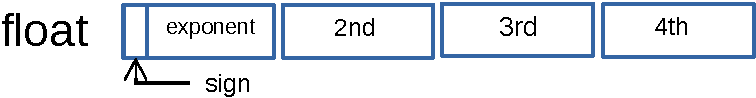
\includegraphics[width=0.5\linewidth]{figs/float.pdf}
	\end{figure}
	[\textbf{3.14159}]
	\begin{lstlisting}[language=c, numbers=none, basicstyle=\small, rulecolor=\color{black}]
	    0 0000100 110010010000111111001110
    ^     ^               ^
    |     |               |
    |     |               +--- significand = 0.7853975
    |     |
    |     +------------------- exponent = 4
    |
    +------------------------- sign = 0 (positive)
	\end{lstlisting}
	
\end{frame}

\begin{frame}[fragile]{Floating point numbers (2)}
	\begin{itemize}
		\item Keywords: \textcolor{blue}{float}, \textcolor{blue}{double}, \textcolor{blue}{long double}
	\end{itemize}
	\begin{lstlisting}[numbers=none, frame=none, language=c]
		float x = 0.125;			/*Precision: 7 to 8 digits*/
		double y = 111111.111111;	/*Precision: 15 to 16 digits*/
	\end{lstlisting}
	\vspace{-0.05in}
	\begin{itemize}
		\item {Now you should know a very useful operator \textcolor{blue}{sizeof}(.)}
	\end{itemize}
	\begin{lstlisting}[numbers=none, frame=none, language=c]
#include <stdio.h>
int main()
{
	float x = 0.125;
	double y = 111111.111111;
	printf("float: %d, double: %d", sizeof(x), sizeof(y));
}
	\end{lstlisting}
\end{frame}

\begin{frame}[fragile]{Characters (1)}
	\begin{itemize}
		\item Keyword: \textcolor{blue}{char}
		\item Can be \textcolor{red}{signed} (default) or \textcolor{blue}{unsigned}	
		\item Size: 1 Byte (8 bits) on almost every architecture
		\item Intended to represent a single character
		\item Stores its \textit{ASCII} number (e.g. 'A' $\Rightarrow$ 65)
	\end{itemize}
	\begin{itemize}
		\item {	You can define a \textcolor{blue}{char} either by its ASCII number or by its symbol:}	
	\end{itemize}
	\begin{lstlisting}[numbers=none, language=c]
		char a = 65;
		char b = 'A';	/*use single quotation marks*/
\end{lstlisting}
\end{frame}

\begin{frame}[fragile]{Characters (2)}
	\begin{itemize}
		\item {Essentially, \textcolor{blue}{char} uses 1 byte to represent 255 characters}
		\item {Each integer is associated with a character}
		\item {American Standard Code for Information Interchange (ASCII)}
	\end{itemize}
	\vspace{-0.06in}
	\begin{figure}
		\centering
		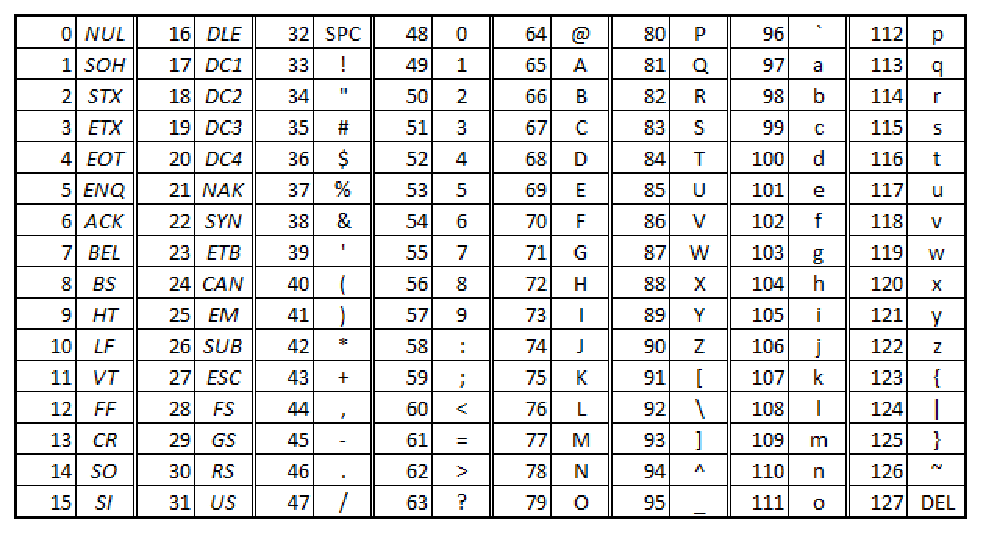
\includegraphics[width=0.8\linewidth]{figs/ascii.pdf}
	\end{figure}
\end{frame}

\begin{frame}[fragile]{Characters (3)}
	\begin{itemize}
		\item {There are some frequently used ones you should know}
	\end{itemize}
\begin{table}
\begin{tabular}{|c|c||c|c|}
\hline
ASCII & value & ASCII & value  \\ \hline
0$\sim$9 & 48$\sim$57 & A$\sim$Z & 65$\sim$90 \\ \hline
 a$\sim$z & 97$\sim$122 & $\llcorner\_\lrcorner$ & 32 \\ \hline
$\setminus$n & 10 & $\setminus$t & 9 \\ \hline
\end{tabular}
\end{table}
\begin{columns}
\begin{column}{0.60\linewidth}
	[\textbf{Code}]
	\begin{lstlisting}[language=c, numbers=none]
#include <stdio.h>
int main()
{
   printf("A: %d %c\n", 'A', 'A');
   printf("1: %d %c\n", '1', '1');
   printf("B: %d %c\n", 66, 66);
   printf("2: %d %c\n", 50, 50);
}
	\end{lstlisting}
\end{column}
\begin{column}{0.35\linewidth}
	[\textbf{Output}]
	\begin{lstlisting}[language=c, numbers=none]
	
	
	
	A: 65 A
	1: 49 1
	B: 66 B
	2: 50 2
	
	
	\end{lstlisting}
\end{column}
\end{columns}
\end{frame}

\begin{frame}[fragile]{Data type and its size}
\begin{figure}
	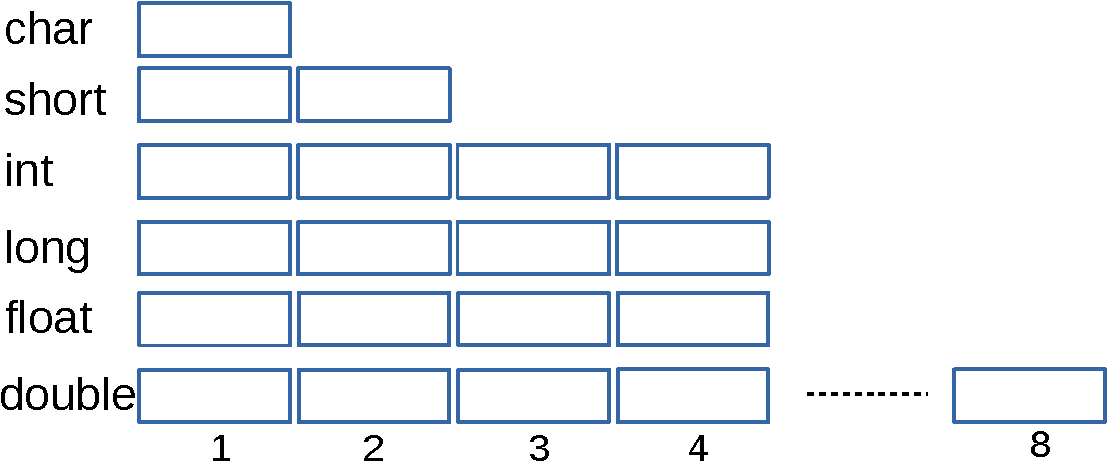
\includegraphics[width=0.85\linewidth]{figs/types.pdf}
\end{figure}
\begin{itemize}
	\item {You should clearly know what is the use of your data}
	\item {One should not define data in double/long double just for convenience}
	\item {It wastes a lot of memory}
	\item {String: an \textbf{array} of chars}
\end{itemize}
\end{frame}